%------------------------------------------------
% Quick reference.
%------------------------------------------------
%
% Для вставки картинок:
%
%--------         Комманда
%
%\begin{figure}[H]
%	\includegraphics{img_name}
%	\caption{some caption}
%	\label{some_pic}
%\end{figure}
%
%--------        Переменные
%
% img_name     <- Название картинки в папке img.
% some_caption <- подпись картинки.
% label        <- лейбл нужен для ссылок на картинку.
% H            <- расположение картинки на странице.
% Чтобы сентрировать добавьте параметр \centering перед строчкой \includegraphics{}
% Чтобы вместить большой рисунок добавьте [width=\textwidth,height=\textheight,keepaspectratio] как параметр к \includegraphics{}
%--------         Пример
%
%\begin{figure}[H]
%   \centering
%	\includegraphics[width=\textwidth,height=\textheight,keepaspectratio]{pic1.jpg}
%	\caption{График зависимости}
%	\label{grapics1}
%\end{figure}
%
%------------------------------------------------
%
% Для референса по лейблу:
%
%--------         Комманда
%
% Для ссылки используется \eqref{ref}.
%
%--------        Переменные
%
% ref          <- указанный лейбл в директиве \label{ref}
%                 Ссылку можно сделать на любой объект имеющий \label{•}
%
%--------         Пример
%
% \eqref{graphics1}
%
%------------------------------------------------
%
% Для листинга кода:
%
%--------         Комманда
%
% \lstinputlisting[language=lang,mathescape=true]{src}
%--------        Переменные
%
% lang         <- язык на котором написан исходный код, например "python" или "C++".
% mathescape   <- если в исходниках есть формулы LaTeX, то они будут представлены как формулы.
% src          <- путь до файла исходников.
%
%--------         Пример
%
% \lstinputlisting[language=C++,mathescape=false]{./src/bullshit.cpp}
%
%------------------------------------------------
%
% Для вставки таблиц:
%
%--------
%\begin{table}[H]
%	\centering
%	\caption{ capt }
%	\begin{tabularx}{0.9\textwidth}{ | Y | Y | }
%		\hline
%		lines
%	\end{tabularx}
%	\label{tab1}
%\end{table}
%--------
% caption      <- Подпись таблицы.
% tab1         <- лейбл нужный для ссылки на таблицу.
% | Y | Y |    <- количество и формат столбцов.
% Y            <- Тип столбца.
%                 В данном случае определены кастомные столбцы Y (Спасибо Максиму Наумову)
% |            <- обозначает границы столбца.
%                 То есть, если будет указано |Y Y|, то столбцы внутри строк разделены не будут.
% H            <- То же самое, что и у картинок.
% lines        <- непосредственно элементы таблицы.
%                 Разделяются знаком "&", оканчивать каждую строку лучше \\ \hline
%
%--------         Пример
%\begin{table}[H]
%	\centering
%	\caption{ capt }
%	\begin{tabularx}{0.9\textwidth}{ | Y | Y | }
%		\hline
%		str1 & str2 \\ \hline
%		str1 & str2 \\ \hline
%		str1 & str2 \\ \hline
%		str1 & str2 \\ \hline
%		str1 & str2 \\ \hline
%	\end{tabularx}
%	\label{tab1}
%\end{table}
%------------------------------------------------

\documentclass[12pt, fleqn]{article}

\makeatletter
\renewcommand*\l@section{\@dottedtocline{1}{1.5em}{2.3em}}



%\includegraphics{universe}
\usepackage[none]{hyphenat}
\usepackage[utf8]{inputenc}
\usepackage[T2A]{fontenc}
\usepackage[russian]{babel} % указывает язык документа
\usepackage[left=3cm,right=2cm,top=2cm,bottom=2cm,bindingoffset=0cm]{geometry}
\usepackage{lastpage}
\usepackage{fancyhdr}
\usepackage{titlesec}
\usepackage{graphicx} % для вставки картинок
\usepackage[intlimits]{mathtools} % математические дополнения
\usepackage{amssymb}
\usepackage[tableposition=top]{caption}
\usepackage{subcaption}
\usepackage{indentfirst}
%\usepackage{pythonhighlight}
\usepackage{listings}
\usepackage{tabularx}
\usepackage{tabulary}
\usepackage{multirow}
\usepackage{float}
\usepackage[figure,table]{totalcount}
\usepackage{diagbox}
\usepackage[german=guillemets]{csquotes}
\usepackage{fontspec}
\usepackage{enumitem}
%\usepackage{mathptmx}% http://ctan.org/pkg/mathptmx
%\usepackage{showframe}
\usepackage{hyperref}
\usepackage{hyphenat}
\usepackage{icomma}
\usepackage{tikz}
\newcommand*\circled[1]{\tikz[baseline=(char.base)]{
   \node[shape=circle,draw,inner sep=1pt] (char) {#1};}}

\setlength{\parindent}{1.2cm}

\setlength{\mathindent}{1.2cm}

\defaultfontfeatures{Ligatures={TeX},Renderer=Basic}
\setmainfont[Ligatures={TeX,Historic}]{Times New Roman}

%\setlist[enumerate]{itemindent=\dimexpr\labelwidth+\labelsep\relax,leftmargin=0pt}

%\setlength{\section*}{0.5cm}
%\usepackage{minted}
%\usepackage{fancyvrb}
%\usepackage{newtxtext}

%\titleformat{\section}[hang]{\bfseries\LARGE\centering}{}{1em}{}

%\setlist[enumerate]{itemindent=\dimexpr\labelwidth+\labelsep\relax,leftmargin=0pt}
\setlist[enumerate,itemize]{leftmargin=0pt,itemindent=1.7cm}
\titleformat{\section}{\large\bfseries\centering}{\thesection}{0.5em}{\MakeUppercase}
\titleformat{\subsection}[block]{\bfseries\hspace{1em}}{\thesubsection}{0.5em}{}
%\setlength{\subsection*}{1.5cm}
%\setlength{\parindent}{4em}

%\setlength{\parindent}{1.5cm}

\captionsetup[figure]{labelfont={it},textfont={it},name={Рисунок},labelsep=endash, skip=5pt}
\captionsetup[table]{labelfont={it},textfont={it},name={Таблица},labelsep=endash,singlelinecheck=false, skip=5pt, margin=1cm}


%\renewcommand{\baselinestretch}{1.5}
\linespread{1.5} % полуторный интервал
\frenchspacing
\graphicspath{ {images/} }

  %-------------------------------------------
  % Переменные
  %-------------------------------------------

  \newcommand{\firstAuthorSurName}{Белоусов} 					                           % Фамилия автора.
  \newcommand{\firstAuthorInitials}{ А. А.} 					                           % Фамилия автора.
  \newcommand{\leftcolon}{Оптоинформационные технологии и системы}
  \newcommand{\teacherName}{Кириленко М.С.}				                               % Имя преподавателя.
  \newcommand{\variantNumber}{9} 							                           % Номер варианта.
  \newcommand{\groupNumber}{6409-010302D} 				                               % Номер группы.
  \newcommand{\subjectTitle}{Оптоинформационные технологии и системы}                                  % Название предмета.
  \newcommand{\taskTitle}{Численная реализация оптического преобразования Фурье на основе быстрого преобразования Фурье}  % Название работы.
  \newcommand{\theme}{Отчет по лабораторной работе №2} 		  % Название работы.

  %-------------------------------------------
  % Ссылки в оглавлении
  %-------------------------------------------


\hypersetup{
    colorlinks,
    citecolor=black,
    filecolor=black,
    linkcolor=black,
    urlcolor=black
}

  %-------------------------------------------
  % Стиль футеров и хедеров
  %-------------------------------------------

\pagestyle{fancy}
\fancyhead[L, R]{}
\fancyfoot[L]{}
\fancyfoot[R]{}
\renewcommand{\footrulewidth}{0pt}
\renewcommand{\headrulewidth}{0pt}

% \renewcommand\subsectionfont{\normalfont\normalsize\bfseries}

\def\l@subsection{\@dottedtocline{2}{3.8em}{3.2em}}

% Для листинга

\lstset{
basicstyle=\footnotesize\ttfamily,
columns=fullflexible,
keywordstyle=\color{blue},
%frame=single,
breaklines=true,
numberstyle=\tiny\color{mygray},
postbreak=\mbox{\textcolor{red}{$\hookrightarrow$}\space},
showstringspaces=false,
}

\newcolumntype{Y}{>{\centering\arraybackslash}X}
\renewcommand{\tabularxcolumn}[1]{m{#1}} % Для вертикального центрировая табличных ячеек.

\begin{document}

%----------------------------------------------------------------------------------------
%	TITLE PAGE
%----------------------------------------------------------------------------------------
\pagenumbering{Alph}

\begin{titlepage}

	\center

	%------------------------------------------------
	%	Заголовки
	%------------------------------------------------

	\textsc{Министерство науки и высшего образования Российской Федерации}\\[-0.15cm]
	\textsc{Федеральное государственное автономное образовательное учреждение}\\[-0.15cm]
	\textsc{высшего образования «Самарский национальный исследовательский}\\[-0.15cm]
	\textsc{университет имени академика С. П. Королева»}\\[-0.15cm]
	\textsc{(Самарский университет)}\\[-0.15cm]

	\textsc{Министерство науки и высшего образования Российской Федерации}\\[1cm]
    {Институт информатики, математики и электроники}\\[-0.2cm]
    {Факультет информатики}\\[-0.2cm]
    {Кафедра технической кибернетики}\\[0.5cm]
	%------------------------------------------------
	%	Название работы
	%------------------------------------------------

	\vfill\vfill


	{\large \textbf{\subjectTitle}}\\[0.3cm]

	{\large \taskTitle}\\[0.5cm]

    {\large \enquote{\textbf{\theme}}}\\[0.5cm]

    \vfill
     
     {Вариант № \variantNumber}\\[0.5cm]

	\vfill\vfill

	\begin{minipage}{1\textwidth}
		\begin{center}
			\begin{tabularx}{\textwidth}{X l}
				Выполнил студент:        & \firstAuthorSurName \firstAuthorInitials \\
				Группа:                  & \groupNumber                     		   \\
				Преподаватель:           & \teacherName         		                \\
			\end{tabularx}
		\end{center}
	\end{minipage}


	%------------------------------------------------
	%	Дата
	%------------------------------------------------

	\vfill\vfill\vfill

	{\centering Самара \the\year}


\end{titlepage}

\pagenumbering{arabic}

\setcounter{page}{2}


%------------------------------------------------
%Задание
%------------------------------------------------

\section*{Задание}
{
	\begin{enumerate}
	    \item Реализовать одномерное финитное преобразование Фурье с помощью
применения алгоритма БПФ.

	\item Построить график гауссова пучка $\mathrm{e}^{-x^2}$. Здесь и далее для каждого графика следует строить отдельно графики амплитуды и фазы. Амплитуда находится как модуль каждого значения функции, фаза -- как аргумент (или с помощью функции atan2).

	\item Убедиться в правильности реализации преобразования, подав на вход гауссов пучок $\mathrm{e}^{-x^2}$ -- собственную функцию преобразования Фурье. На выходе тоже должен получиться гауссов пучок (построить график на правильной области определения $[-\tilde{b}, \tilde{b}]$). Рекомендуемая входная область: $[−a, a]$ = $[−5, 5]$.

	\item Реализовать финитное преобразование Фурье стандартным методом численного интегрирования (например, методом прямоугольников). Важно: необходимо вычислить интеграл для каждого дискретного значения $u$, чтобы получить результат в виде вектора. На вход преобразования вновь следует подавать гауссов пучок.

	\item Построить результаты двух разных реализаций преобразования на одном изображении (одно для амплитуды, одно для фазы) и убедиться, что они совпадают.
	
	\item Используя первую реализацию преобразования, подать на вход световое поле, отличное от гауссова пучка, в соответствии со своим вариантом. Построить графики самого пучка и результата преобразования.
	
	\item Рассчитать аналитически результат преобразования своего варианта поля и построить график на одной системе координат с результатом, полученным в предыдущем пункте.
	\end{enumerate}
}
\newpage

\section*{Алгоритм реализации оптического финитного преобразования Фурье через использование БПФ}
{
	\begin{enumerate}
		\item Провести дискретизацию входной функции $f(x)$ в вектор $f$ с размерностью N.
		\item Дополнить вектор $f$ и слева, и справа необходимым числом нулей до размерности $M$.
		\item Разбить вектор f на две половины и поменять их местами.
		\item Выполнить БПФ от $f$ и умножить результат на шаг $h_x$ , получив вектор $F$.
		\item Разбить вектор $F$ на две половины и поменять их местами.
		\item \enquote{Вырезать} центральную часть вектора $F$, оставив $N$ элементов.
	\end{enumerate}
}
\newpage

\newpage
\tableofcontents
\newpage

%\phantomsection
%\addcontentsline{toc}{section}{Введение}
%------------------------------------------------
%Введение
%------------------------------------------------



%------------------------------------------------
% Начало основной части
%------------------------------------------------
\titleformat{\section}{\large\bfseries}{\thesection}{0.5em}{}
\titlespacing*{\section}{\parindent}{1ex}{1em}

\section{Реализация одномерного финитного преобразования Фурье}
{
    Одномерное финитное преобразование Фурье записывается следующим образом:
    \begin{equation}\label{fin_transform}
        F_a(u) = \Phi_a \left[ f(x) \right] (u) = \int\limits_{-a}^{a} f(x) e^{-2 \pi i x u} \,dx,
    \end{equation}
    	где $f(x)$ -- финитная функция, $F_a(u)$ -- спектр, $\Phi_a$ -- оператор финитного преобразования Фурье.
    	
    	Здесь и далее в работе используется язык программирования Python.
    	
    	Данное преобразование реализуем с использованием функций из пакета fft библиотеки numpy:
    	
    	\begin{lstlisting}[frame=single,language=Python,mathescape=true] 
    	def fourier_builitn(f, step: float, xs: List[float]) -> List[float]:
	    	fs = list(map(lambda x: f(x), xs))
	    	fs = np.fft.fftshift(fs)
	    	fourier = list(map(lambda x: x * step, np.fft.fft(fs)))
	    	return np.fft.fftshift(fourier)
    	\end{lstlisting}
}
\newpage

\section{Построение графика гауссова пучка}
{
    Гауссов пучок определяется следующим образом:
    \begin{equation}
        f(x) = e^{-x^2}
    \end{equation}


    Вычислим преобразование Фурье гауссова пучка. Построим графики амплитуды и фазы следующей функцией:
    %    	\begin{lstlisting}[frame=single,language=Python,mathescape=true]
    %    def plot_function(f, a, b, step_count, fig):
    %            step = (b - a) / step_count
    %            xs = np.arange(a, b, step)
    %            ys = f(xs)
    %            plt.figure(f"Function {fig}")
    %            plt.grid()
    %            plt.plot(xs, ys)
    %    	\end{lstlisting}
    На рисунках ниже представлены результаты работы программы.
    	\begin{figure}[H]
       \centering
            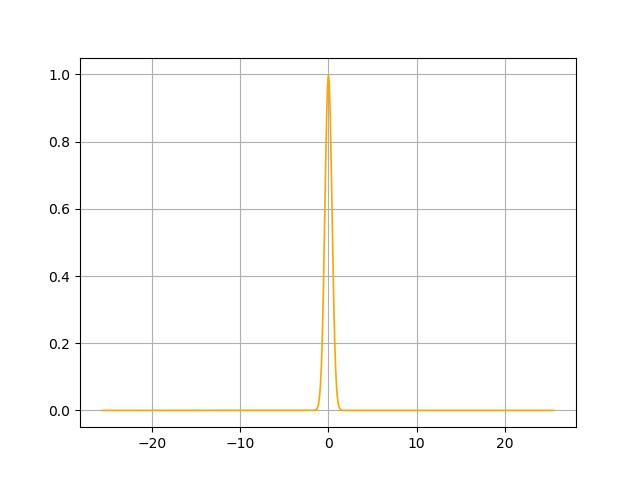
\includegraphics[width=\textwidth,height=\textheight,keepaspectratio]{Gauss_beam_fft.png}
            \caption{График функции гауссова пучка}
            \label{gauss_beam_pic}
    \end{figure}

    	\begin{figure}[H]
       \centering
            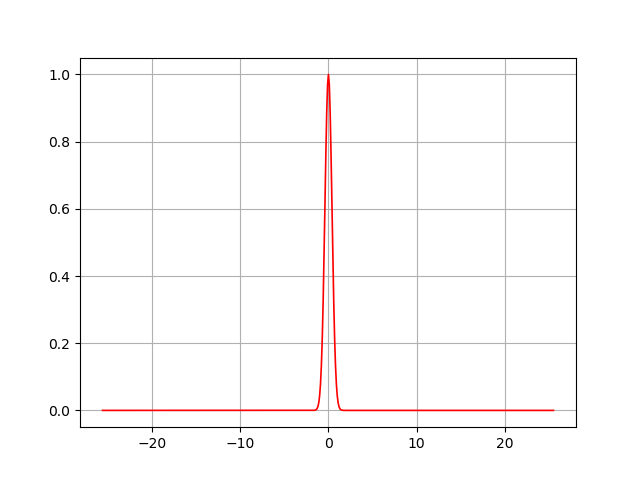
\includegraphics[width=\textwidth,height=\textheight,keepaspectratio]{Gause_beam_amplitude_fft.png}
            \caption{Амплитуда функции гауссова пучка}
            \label{beam_ampl_pic}
    \end{figure}
 
    \begin{figure}[H]
       \centering
            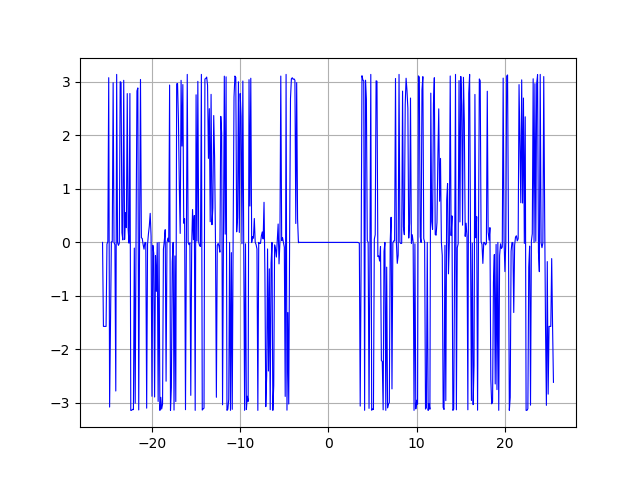
\includegraphics[width=\textwidth,height=\textheight,keepaspectratio]{Gauss_Phase_fft.png}
            \caption{Фаза функции гауссова пучка}
            \label{beam_phase_pic}
    \end{figure}
    
    Для проверки корректности работы программы наложим график исходной функции на график. 
    Амплитуда Гауссова пучка после преобразования должна совпадать с исходной функцией.
    
    \begin{figure}[H]
       \centering
            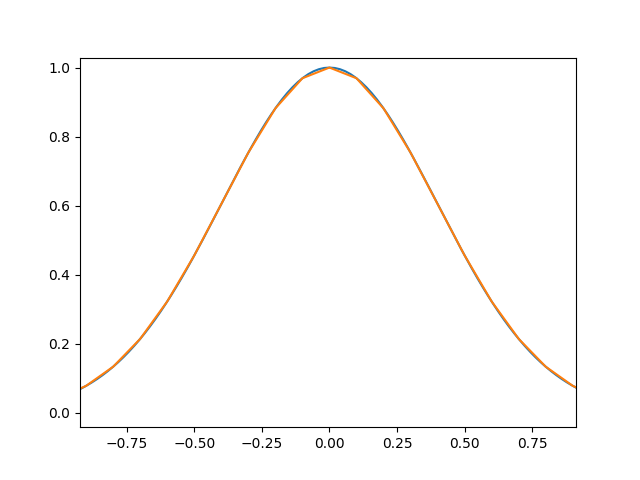
\includegraphics[width=\textwidth,height=\textheight,keepaspectratio]{merged_amplitude_gauss_fft.png}
            \caption{Объединенный график исходной функции и её амплитуды}
            \label{beam_merged_src_amplitude_pic}
    \end{figure}
    Как видно из рисунка \ref{beam_merged_src_amplitude_pic}, графики совпадают с незначительным отклонениями, следовательно преобразование реализовано верно.
    
}

\newpage
\section{Численное финитное преобразование Фурье}
{
    Для реализации численного финитного преобразования воспользуемся методом прямоугольников при численном вычислении определенного интеграла.
    Метод прямоугольников определяется следующим образом:
    \begin{equation}
        \int\limits_a^b{f(x)dx} = \sum_{k=1}^{n}{f\left(\dfrac{x_{i-1} + x_i}{2}(x_i - x_{i-1}) \right)} 
    \end{equation}
    
    Реализуем численное финитное преобразование Фурье используя метод прямоугольников. Конечная программа представлена ниже.
    \begin{lstlisting}[frame=single,language=Python,mathescape=true] 
def calculus_exp(u: float, x: float) -> float:
        """calculus_exp
        Returns $e^{-2 \pi i u x}$ from fourier transform.
        :param u: u value
        :type u: float
        :param x: x value
        :type x: float
        :rtype: float
        """
        return np.exp(-2 * np.pi * 1j * u * x)


def calculus_fourier(f, step: float, xs: [float],
                     us: List[float]) -> List[float]:
        fourier = []
        for u in us:
            newx = 0
            for x in xs:
                newx += f(x) * calculus_exp(u, x)
            newx *= step
            fourier.append(newx)
        return fourier

    	\end{lstlisting}
    	
    	Сравним написанную реализацию численного финитного преобразования Фурье с финитным преобразованием Фурье через БПФ.
    	На рисунках \ref{calc_fft_diff} и \ref{calc_fft_diff_close} показано сравнения реализованных методов.
    	
    	\begin{figure}[H]
       \centering
            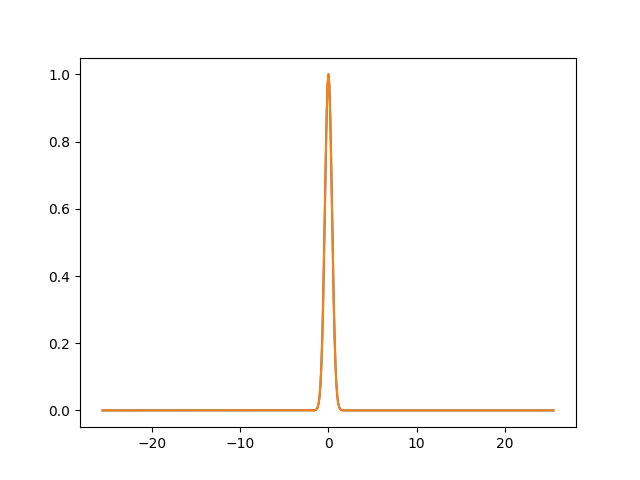
\includegraphics[width=\textwidth,height=\textheight,keepaspectratio]{calc_fft_diff.png}
            \caption{Сравнение численного преобразование Фурье и Фурье через БПФ}
            \label{calc_fft_diff}
    \end{figure}
    
    При достаточном приближении видно, что значения преобразований совпадают, но есть небольшая погрешность  вычисления численным методом. Однако для нашей задачи это не сыграет роли.
    \begin{figure}[H]
       \centering
            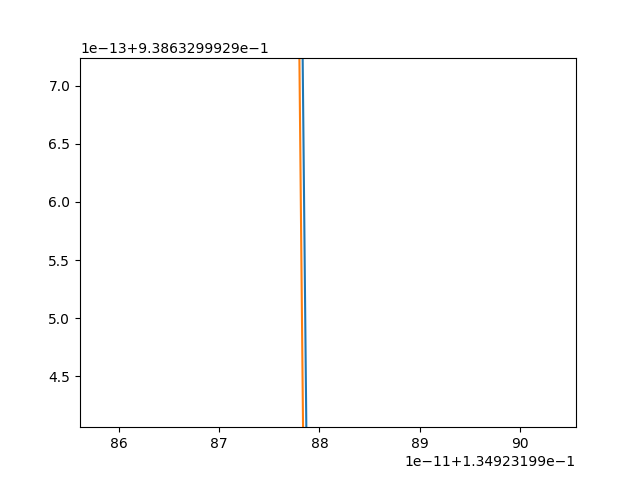
\includegraphics[width=\textwidth,height=\textheight,keepaspectratio]{calc_fft_diff_close.png}
            \caption{Сравнение численного преобразование Фурье и Фурье через БПФ в приближении}
            \label{calc_fft_diff_close}
    \end{figure}
}

\newpage
\section{Построение функции по варианту}{
    Дана функция 
    \begin{equation}\label{bokunofun}
        f(x) = e^{2 \pi i x} + e^{-5 \pi i x}
    \end{equation}
    Построим для функции \eqref{bokunofun} графики преобразования Фурье через БПФ. 
    На рисунках ниже показаны амплитуда и фаза исходной и преобразованной функции.
    
    \begin{figure}[H]
       \centering
            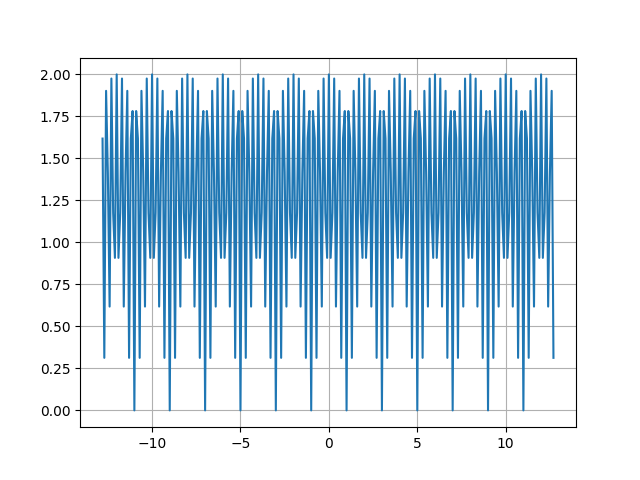
\includegraphics[width=\textwidth,height=\textheight,keepaspectratio]{Amplitude_bokunosource.png}
            \caption{Амплитуда исходной функции}
            \label{bokunoamplitude}
    \end{figure}
    
    \begin{figure}[H]
       \centering
            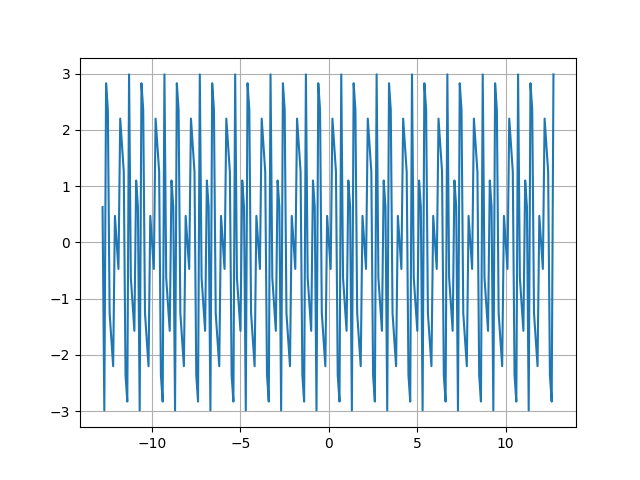
\includegraphics[width=\textwidth,height=\textheight,keepaspectratio]{Phase_bokunosource.png}
            \caption{Фаза исходной функции}
            \label{bokunophase}
    \end{figure}

    \begin{figure}[H]
       \centering
            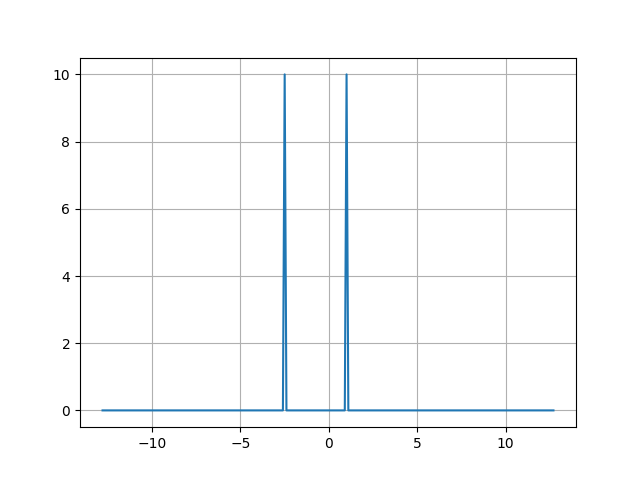
\includegraphics[width=\textwidth,height=\textheight,keepaspectratio]{Amplitude_bokunofft.png}
            \caption{Амплитуда преобразованной функции}
            \label{bokunofourieramplitude}
    \end{figure}
    
    \begin{figure}[H]
       \centering
            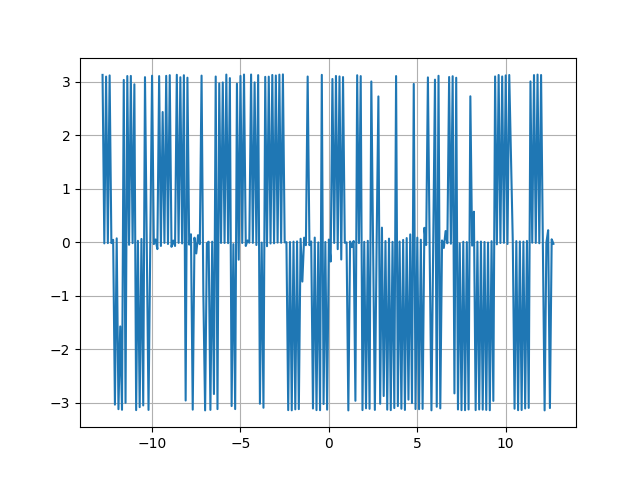
\includegraphics[width=\textwidth,height=\textheight,keepaspectratio]{Phase_bokunofft.png}
            \caption{Фаза преобразованной функции}
            \label{bokunofourierphase}
    \end{figure}
}

\newpage
\section{Построение аналитической функции по варианту}{
	Для функции \eqref{bokunofun} найдем аналитическое преобразование Фурье $(\mathfrak{F}(f(x)))$.
	
	\begin{align*}
	    &e^{2 \pi i x} + e^{-5 \pi i x} \xrightarrow{\mathfrak{F}} \int_{a}^{b}{\left( e^{2 \pi i x} + e^{-5 \pi i x} \right) e^{-2 \pi i x \xi } dx} = \int_{a}^{b}{e^{2 \pi i x} e^{-2 \pi i x \xi } dx} + \int_{a}^{b}{e^{-5 \pi i x} e^{-2 \pi i x \xi } dx} = \\
	    &= \int_{a}^{b}{e^{-2\pi i x (\xi - 1)}dx} + \int_{a}^{b}{e^{-2 \pi i x \left( \xi + \dfrac{5}{2} \right)}dx} = \dfrac{e^{-2\pi i x (\xi - 1)}}{-2\pi i ( \xi - 1)} \bigg|_a^b + \dfrac{e^{-2 \pi i x \left( \xi + \dfrac{5}{2}\right)}}{-2 \pi i \left( \xi + \dfrac{5}{2} \right)} \bigg|_a^b = \\
	    &= \dfrac{ e^{-2\pi i b (\xi - 1)} - e^{-2\pi i a (\xi - 1)} }{-2\pi i ( \xi - 1)} + \dfrac{e^{-2 \pi i b \left( \xi + \dfrac{5}{2}\right)} - e^{-2 \pi i a \left( \xi + \dfrac{5}{2}\right)}}{-2 \pi i \left( \xi + \dfrac{5}{2} \right)}
	\end{align*}
    
    Ниже представлена реализация данной аналитической функции на языке программирования Python.
    \begin{lstlisting}[frame=single,language=Python,mathescape=true] 
    def analit_func(a, b, u):
            """analit_func
                $\dfrac{e^{-2 \pi i b (u-1)} - e^{-2 \pi i a (u-1)}}{-2 \pi i (u-1)} + \dfrac{((e^{-2 \pi i b
                            (u + 2.5)}) - e^{(-2 \pi i a (u + 2.5))})}{(-2 \pi i (u + 2.5))}$
            """
            return (np.exp(-2 * np.pi * 1j * b * (u - 1)) - np.exp(
                -2 * np.pi * 1j * a * (u - 1))) / (-2 * np.pi * 1j * (u - 1)) + (
                (np.exp(-2 * np.pi * 1j * b *
                        (u + 2.5)) - np.exp(-2 * np.pi * 1j * a * (u + 2.5))) /
                (-2 * np.pi * 1j * (u + 2.5)))
    \end{lstlisting}	
	
	На следующих рисунках представлен результат работы аналитического решения и его сравнение с численным решением.
	
	\begin{figure}[H]
       \centering
            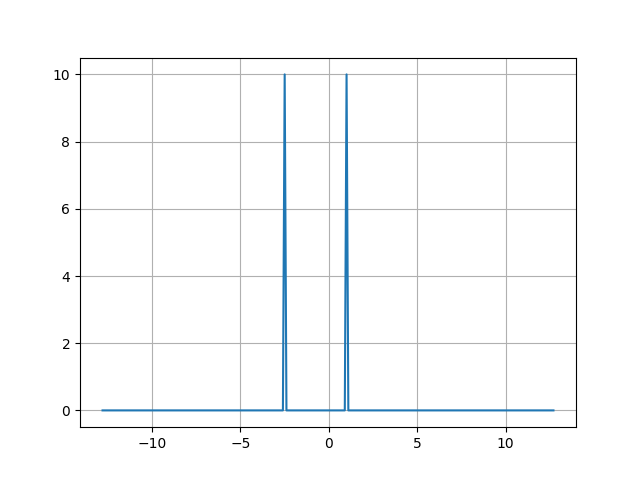
\includegraphics[width=\textwidth,height=\textheight,keepaspectratio]{Amplitude_calc.png}
            \caption{Амплитуда преобразованной функции}
    \end{figure}
    
    \begin{figure}[H]
       \centering
            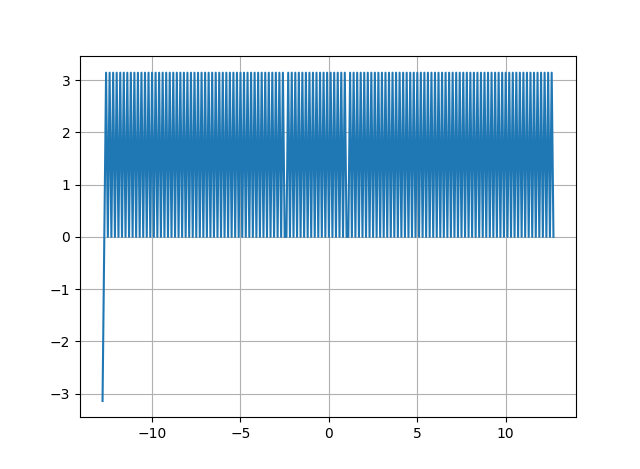
\includegraphics[width=\textwidth,height=\textheight,keepaspectratio]{Phase_calc.png}
            \caption{Амплитуда преобразованной функции}
    \end{figure}
        
    
    \begin{figure}[H]
       \centering
            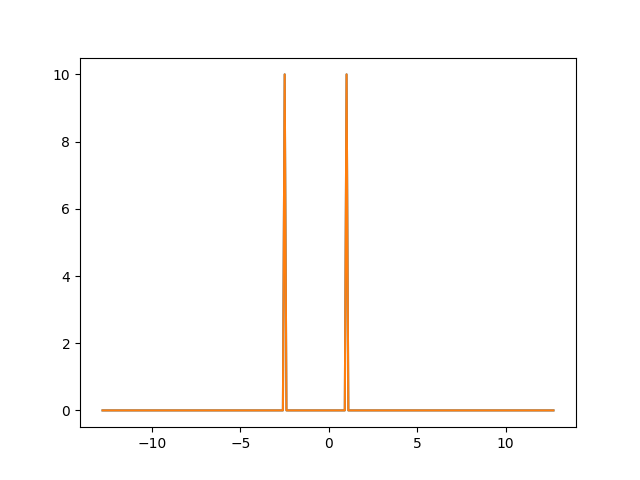
\includegraphics[width=\textwidth,height=\textheight,keepaspectratio]{Amplitude_test.png}
            \caption{Сравнение амплитуды}
    \end{figure}
    
     \begin{figure}[H]
       \centering
            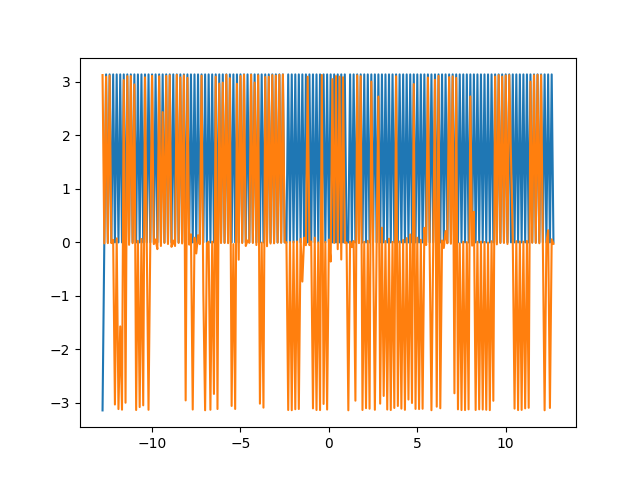
\includegraphics[width=\textwidth,height=\textheight,keepaspectratio]{Phase_test.png}
            \caption{Сравнение фазы}
    \end{figure}
        
    Ниже представлено сравнение графиков в нулевых точках.       
       
    \begin{figure}[H]
       \centering
            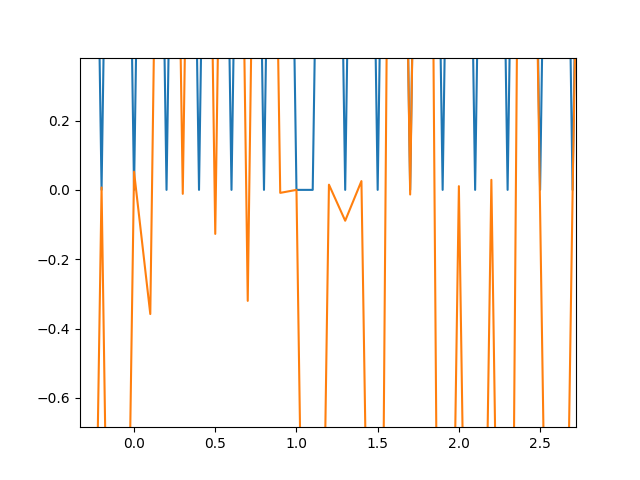
\includegraphics[width=\textwidth,height=\textheight,keepaspectratio]{Phase_test(1).png}
            \caption{Сравнение фазы в точке x=1}
    \end{figure}
    
    \begin{figure}[H]
       \centering
            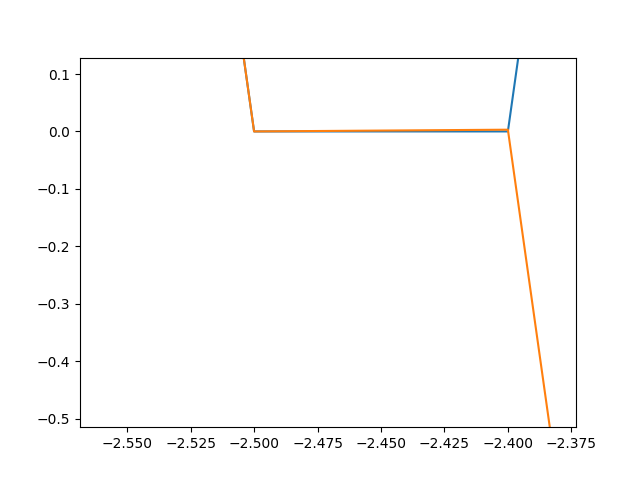
\includegraphics[width=\textwidth,height=\textheight,keepaspectratio]{Phase_test2.png}
            \caption{Сравнение фазы в точке x=-$\dfrac{5}{2}$}
    \end{figure}
}
\titleformat*{\section}{\large\bfseries\centering}

\newpage
\phantomsection
\addcontentsline{toc}{section}{Заключение}

%------------------------------------------------
% Заключение
%------------------------------------------------

\section*{ЗАКЛЮЧЕНИЕ}
{
	В данной лабораторной работе было реализовано одномерное финитное преобразование Фурье с помощью метода БПФ, а так же с помощью метода численного интегрирования. Был рассчитан теоритический результат преобразования Фурье для функции $e^{2 \pi i x} + e^{- 5 \pi i x}$. Построены графики для сравнения результатов различных преобразований. Были найдены результаты аналитического преобразования Фурье и преобразования Фурье через быстрое преобразование Фурье .
}

%\newpage
%\phantomsection
%\addcontentsline{toc}{section}{Список использованных источников}

%------------------------------------------------
% Список литературы
%------------------------------------------------


%------------------------------------------------
% Приложения. Коды программ и.т.д.
%------------------------------------------------

\newpage
\phantomsection
\addcontentsline{toc}{section}{Приложение А Код программы}
\section*{Приложение А}
{
	\begin{center}
	\textbf{Код программы}
	\end{center}
	\lstinputlisting[language=Python,mathescape=true]{./src/main.py}
}
\end{document}
